\section{Resultados}

\subsection{Comunicación Maestro–Esclavo mediante SPI}

La implementación final del circuito SPI se presenta en la Figura~\ref{fig:circuitoSPi}. El sistema operó de forma correcta, obteniéndose el comportamiento esperado. Inicialmente se evaluó mostrar los datos de los sensores mediante USART, pero finalmente se optó por prescindir de ella con el fin de maximizar la velocidad de transmisión y asegurar una respuesta inmediata por parte de los actuadores.

\begin{figure}[H]
    \centering
    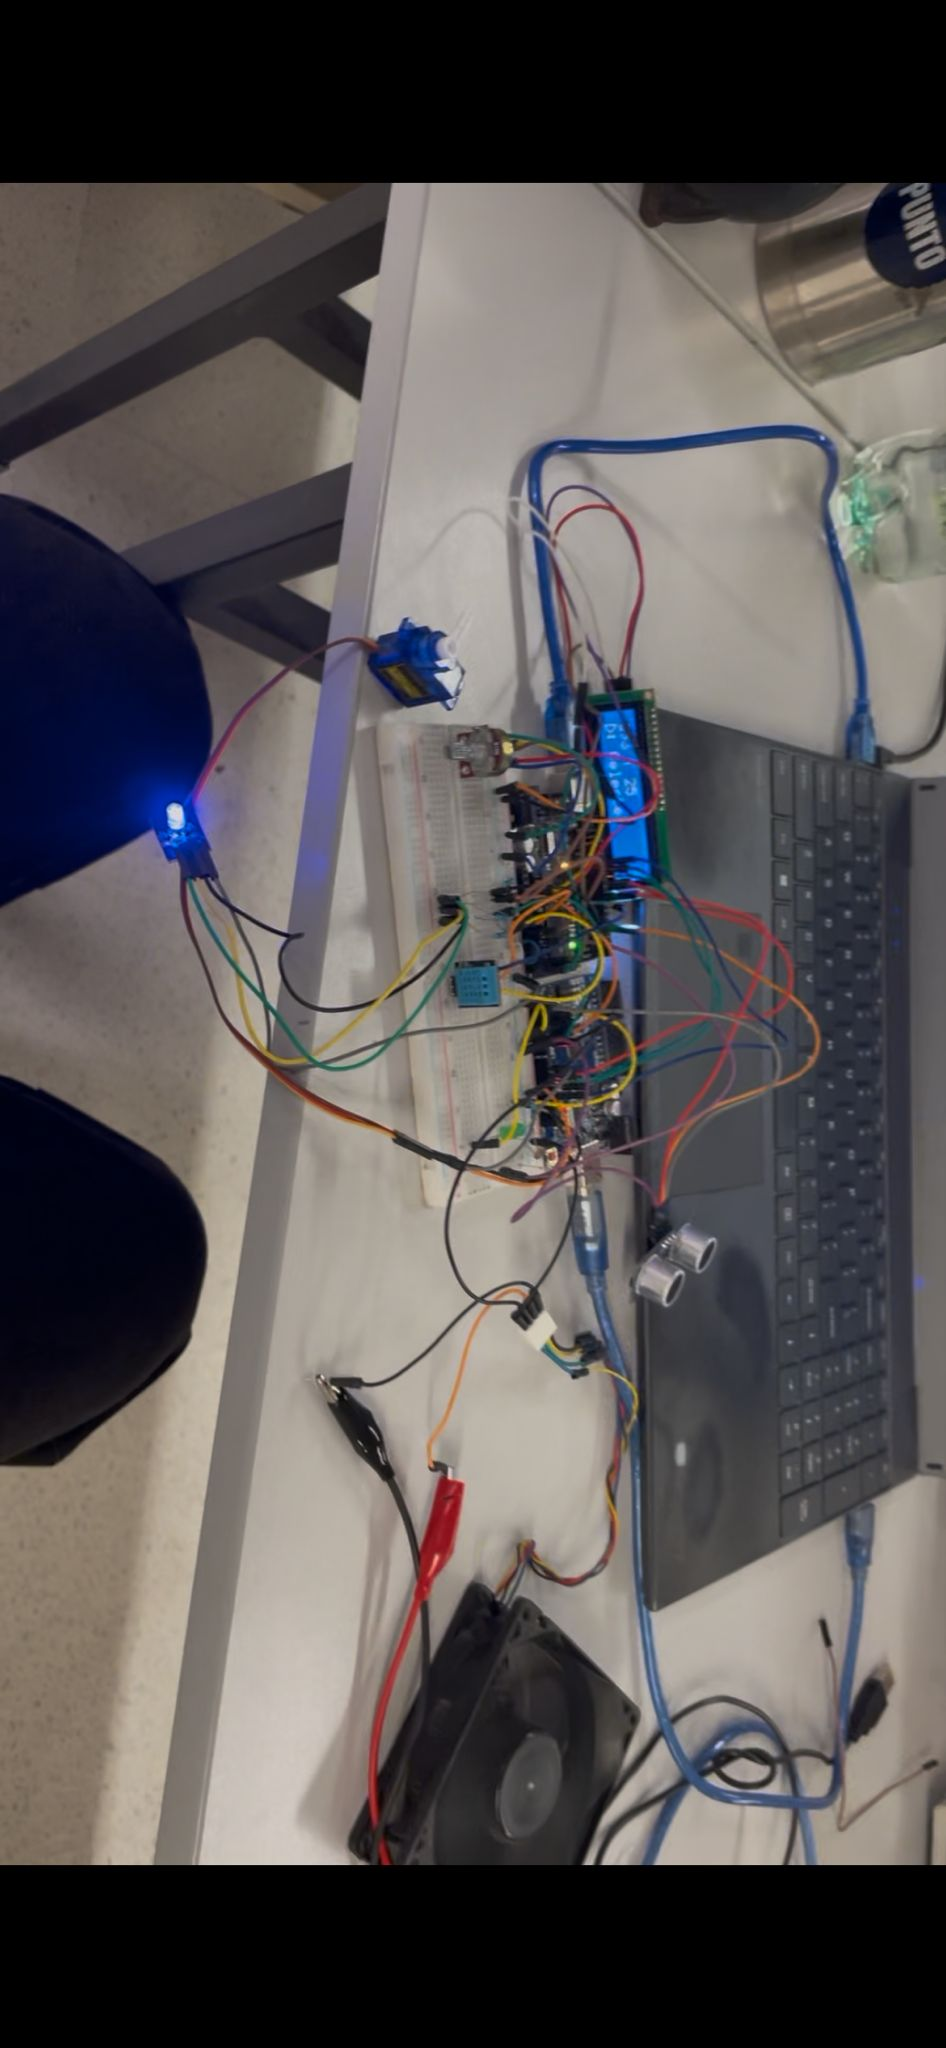
\includegraphics[width=0.45\textwidth]{anexos/1 SPI/WhatsApp Image 2025-11-19 at 19.38.24_0c64da37.jpg}
    \caption{Implementación física del circuito SPI. Fuente: elaboración propia}
    \label{fig:circuitoSPi}
\end{figure}

\subsection{Simulación}

La simulación del sistema se realizó en Proteus, donde se probo el comportamiento del enlace maestro–esclavo. La Figura~\ref{fig:SImcircuitoSPI} muestra la disposición simulada del circuito y la correcta interacción entre los dispositivos.

\begin{figure}[H]
    \centering
    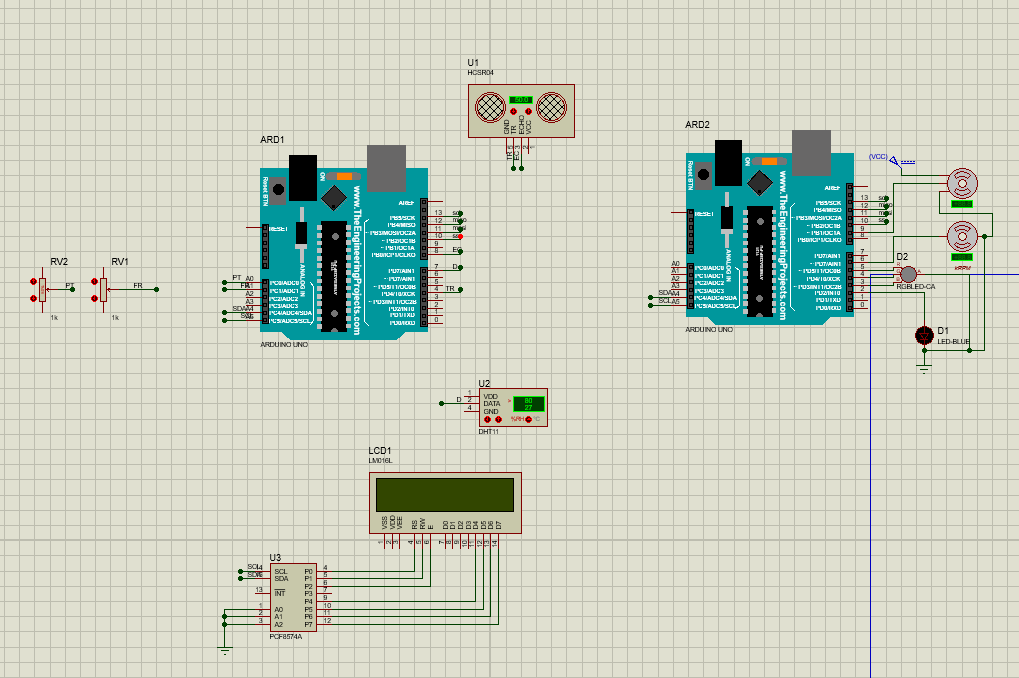
\includegraphics[width=0.45\textwidth]{anexos/1 SPI/aad.png}
    \caption{Implementación simulada del circuito SPI. Fuente: elaboración propia}
    \label{fig:SImcircuitoSPI}
\end{figure}


\subsection{Comunicación Maestro–Esclavo mediante I2C}

La implementación final del circuito I2C Maestro–Esclavo puede observarse en la Figura~\ref{fig:circuitoI2C}. El sistema funcionó correctamente, logrando una transmisión de datos estable y eficiente. Todos los sensores respondieron de forma adecuada, garantizando una actualización inmediata en el dispositivo esclavo.

\begin{figure}[H]
    \centering
    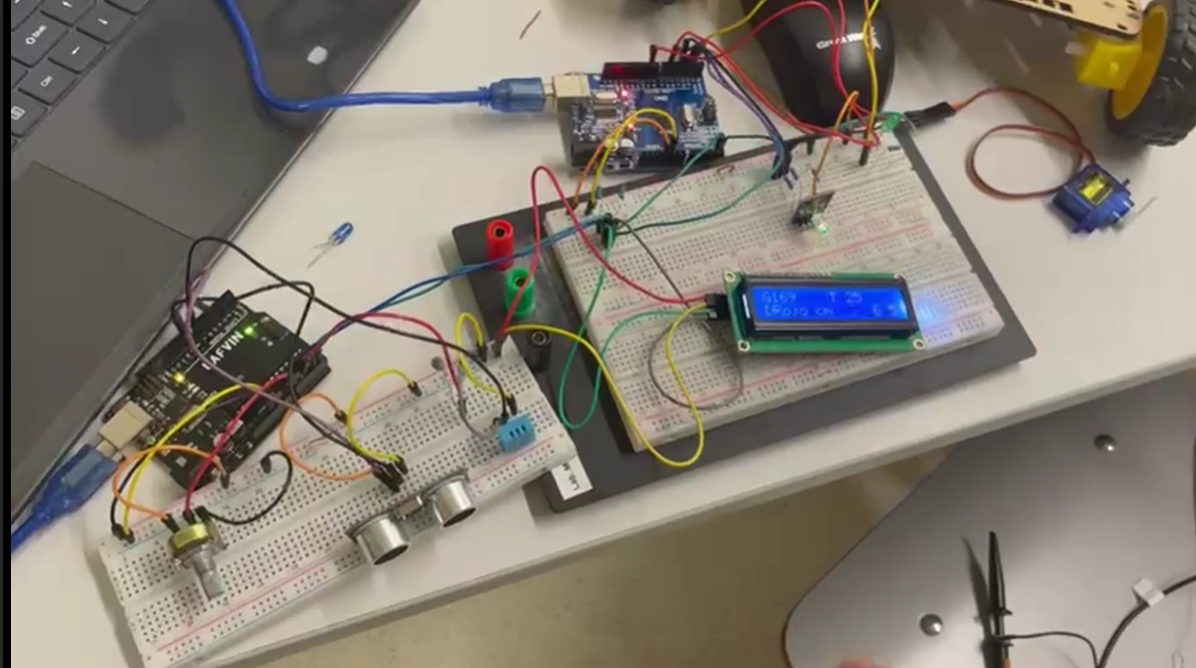
\includegraphics[width=0.45\textwidth]{anexos/2 I2C/I2C.png}
    \caption{Implementación física del circuito I2C. Fuente: elaboración propia}
    \label{fig:circuitoI2C}
\end{figure}

\subsubsection{Simulación}

La simulación del sistema se realizó en Proteus, donde se testeo el comportamiento del enlace maestro–esclavo. La Figura~\ref{fig:SImcircuitoI2C} muestra la disposición simulada del circuito y la correcta interacción entre los dispositivos.

\begin{figure}[H]
    \centering
    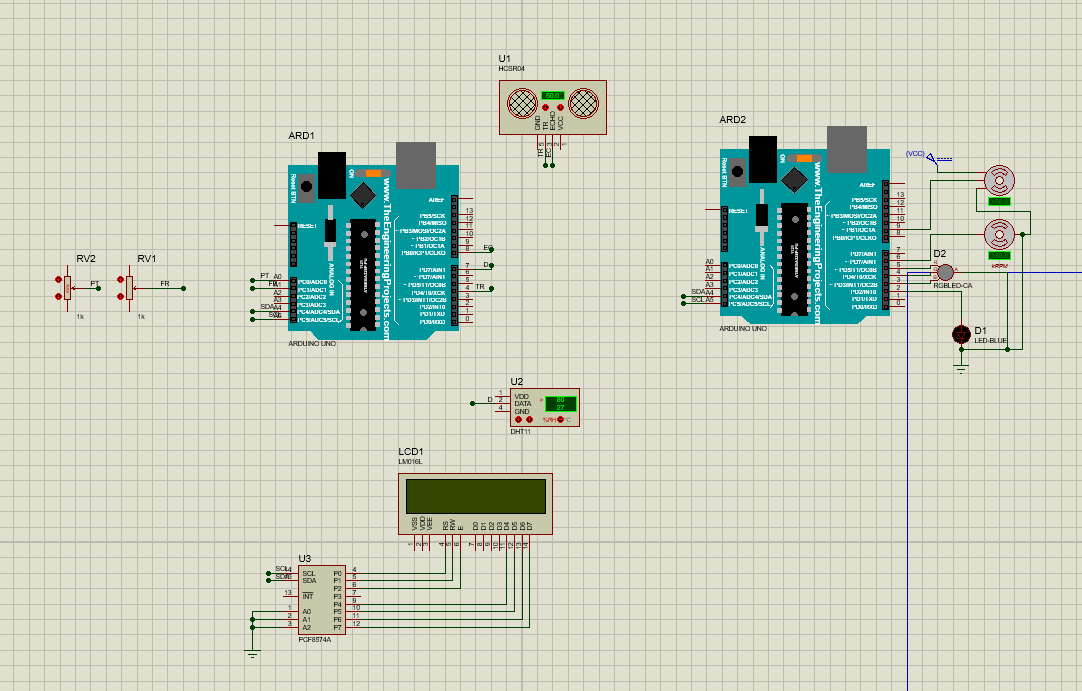
\includegraphics[width=0.45\textwidth]{anexos/2 I2C/image.png}
    \caption{Implementación simulada del circuito I2C. Fuente: elaboración propia}
    \label{fig:SImcircuitoI2C}
\end{figure}

\subsubsection{Visualización de la señal – I2C}

En la Figura~\ref{fig:SigmcircuitoI2C} se presenta la señal capturada mediante el osciloscopio del protocolo I2C. Se observa la transferencia de datos sincronizada con la línea de reloj (SCL). Además, se adjunta en el repositorio del laboratorio un video demostrativo donde se aprecia la comunicación en tiempo real.

\begin{figure}[H]
    \centering
    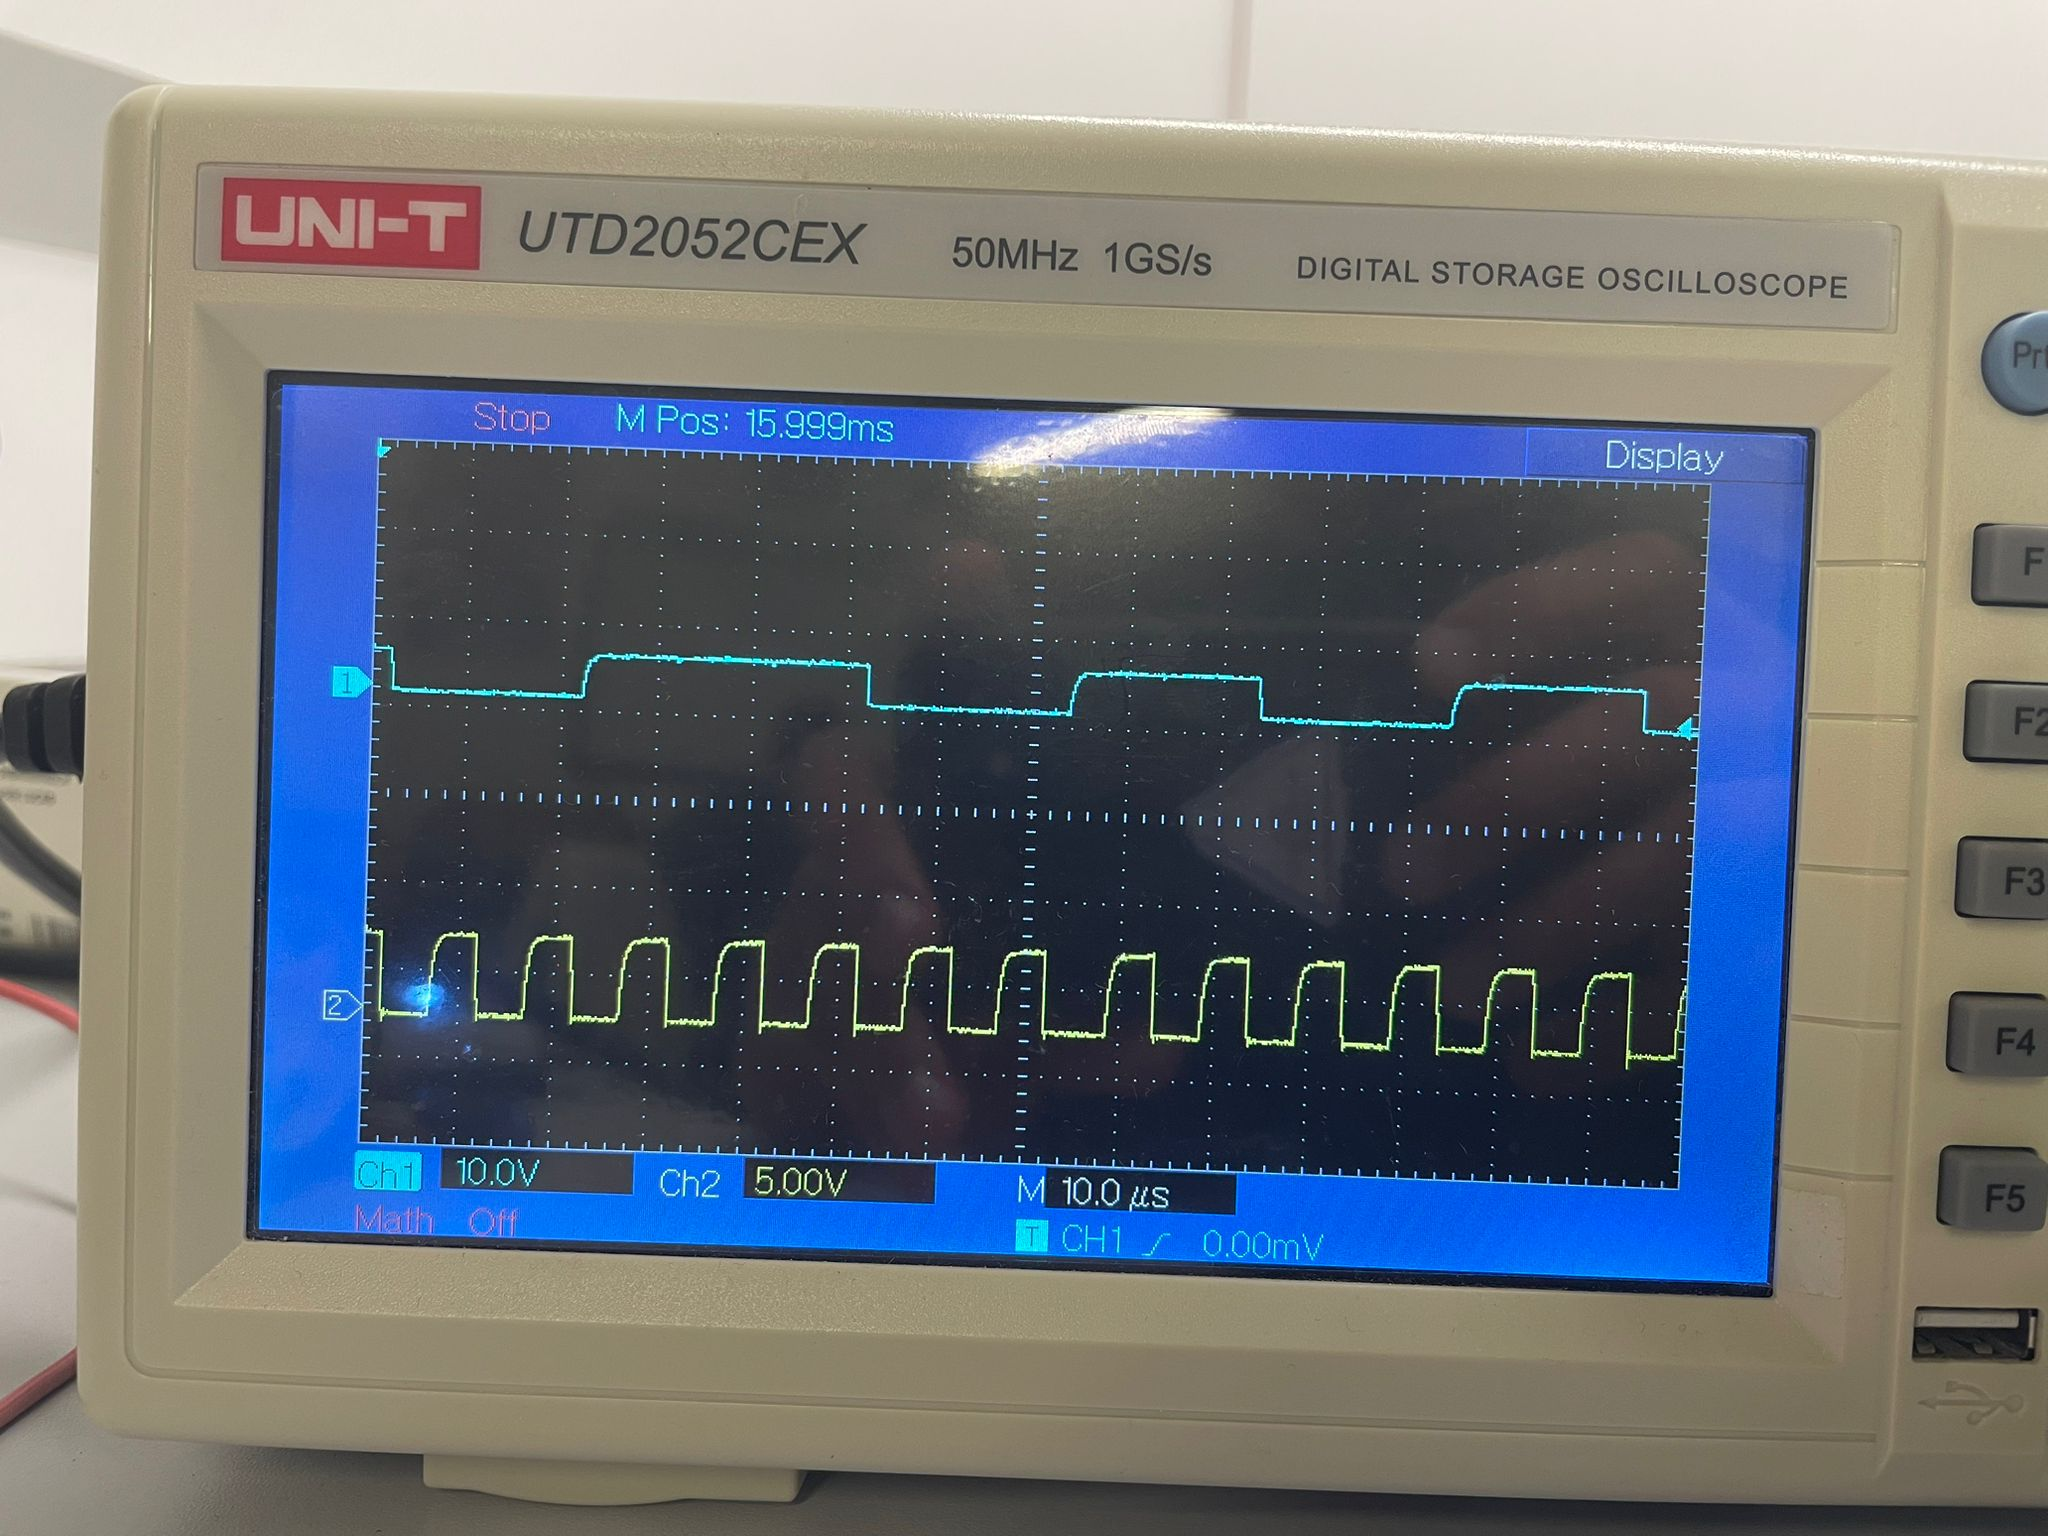
\includegraphics[width=0.45\textwidth]{anexos/2 I2C/I2Csigna.jpg}
    \caption{Captura de la señal del bus I2C. Fuente: elaboración propia}
    \label{fig:SigmcircuitoI2C}
\end{figure}


\subsection{Auto - Futbol}

La implementación final de auto se puede ver en la figura \ref{fig:FisicoAuto}. Se uso una extension de MDF para el golpe del motor, un Power-bank para la alimentacion y dos motores de corriente continua para el movimiento. 

\begin{figure}[H]
    \centering
    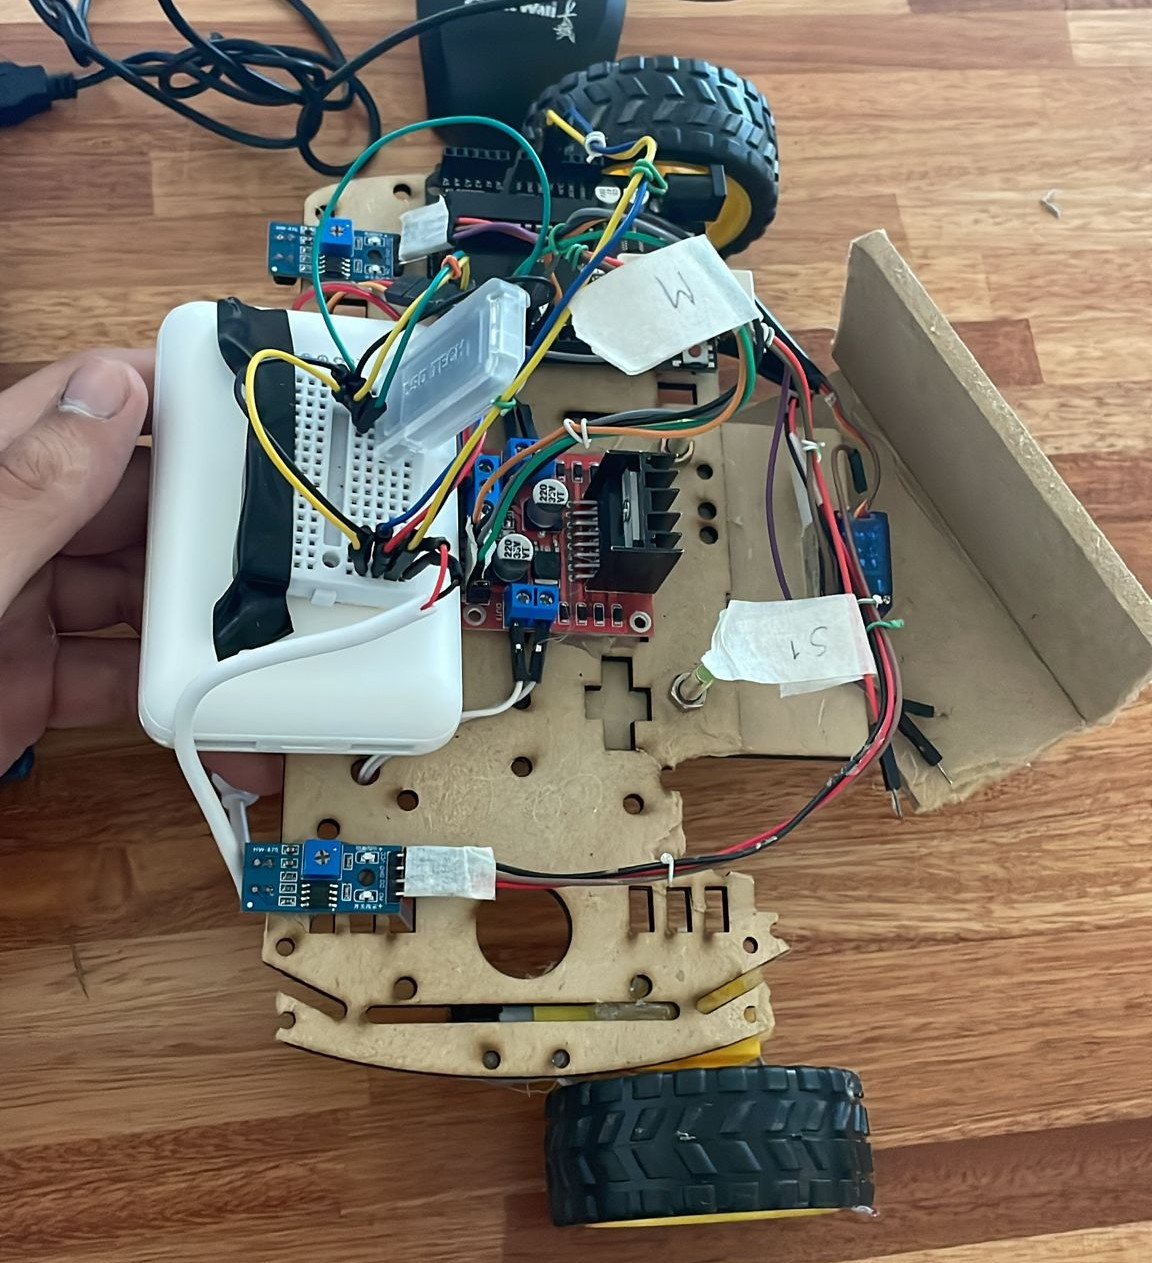
\includegraphics[width=0.45\textwidth]{anexos/5 Futbol/Fisico.jpg}
    \caption{Implementacion Fisica Auto. Fuente: elaboración propia}
    \label{fig:FisicoAuto}
\end{figure}

Funcionó correctamente y no hubo problemas en su implementación.

\subsubsection{Comunicación Bluetooth}

Para la comunicación Bluetooth se uso la aplicacion, se puede ver una imagen de la interfaz y los comandos mandados en las fguras \ref{fig:App} y \ref{fig:Appc} respectivamente.

\begin{figure}[H]
    \centering
    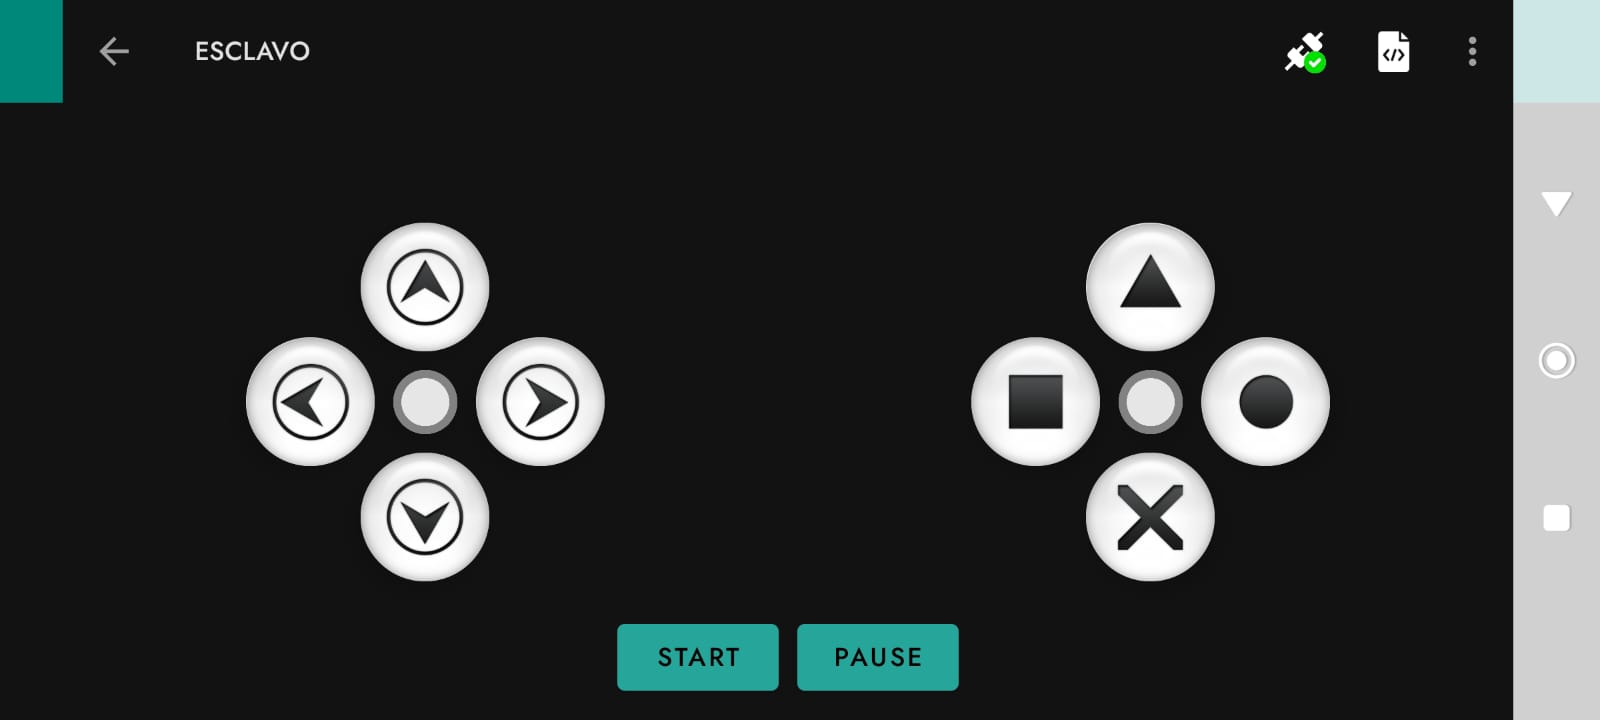
\includegraphics[width=0.45\textwidth]{anexos/5 Futbol/App.jpg}
    \caption{Aplicacion para manejo de auto. Fuente: elaboración propia}
    \label{fig:App}
\end{figure}


\begin{figure}[H]
    \centering
    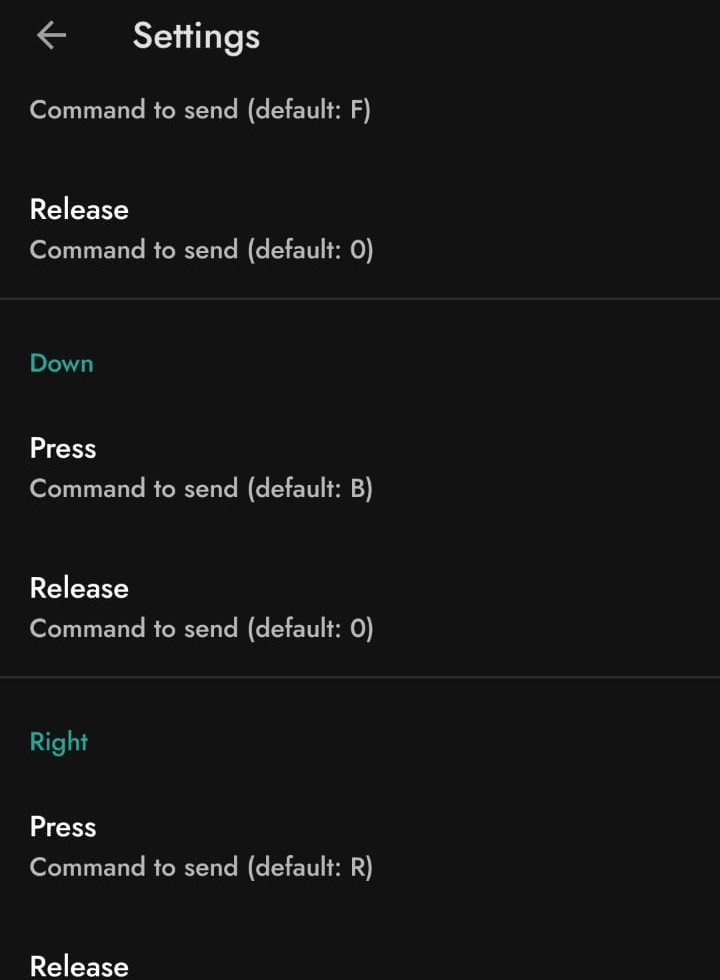
\includegraphics[width=0.3\textwidth]{anexos/5 Futbol/Comandos.jpg}
    \caption{Comandos de la aplicacion. Fuente: elaboración propia}
    \label{fig:Appc}
\end{figure}


\subsection{Control y Animaciones en Matriz WS2812}

La animación arcoíris diagonal se ejecutó de manera fluida sobre la matriz WS2812, sin presentar parpadeos, cortes ni variaciones de brillo. El patrón mantuvo una transición suave de colores y el desplazamiento diagonal se observó tal como se había diseñado, con una correcta interpretación del generador de gradiente \texttt{wheel\_color()}. El brillo de los LEDs se mantuvo homogéneo a lo largo de toda la matriz, sin zonas apagadas ni saturaciones perceptibles. 

Además, el sistema respondió inmediatamente a los comandos USART, permitiendo interrumpir o cambiar la animación sin retrasos. Esto permitió validar la robustez del protocolo WS2812 incluso bajo cambios bruscos de rutina.

\begin{figure}[H]
    \centering
    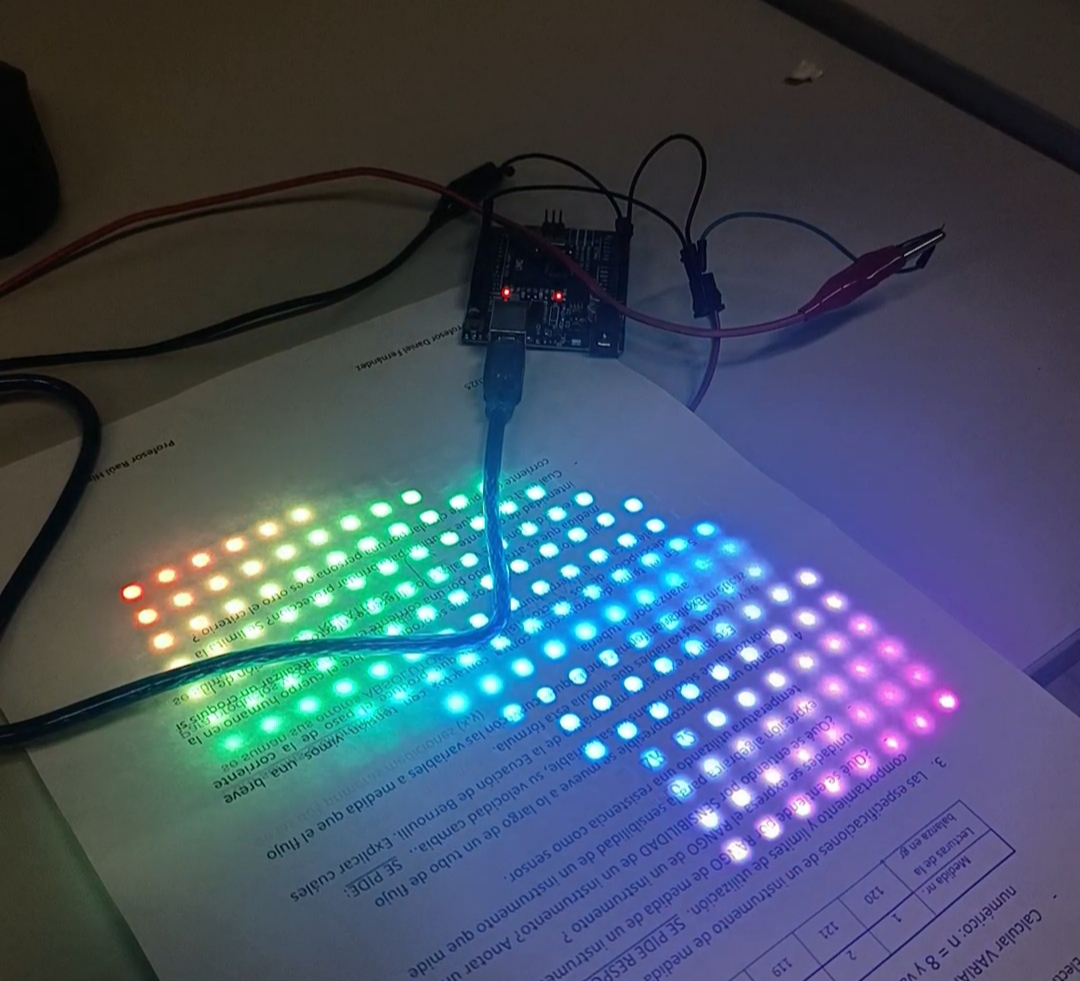
\includegraphics[width=0.45\textwidth]{anexos/3 Animacion/arcoiris.jpg}
    \caption{Funcionamiento general del sistema: animación arcoíris en la matriz WS2812. Fuente: elaboración propia}
    \label{fig:WSanim}
\end{figure}

\subsection{Control de Movimiento en Matriz WS2812 mediante MPU6050}

Durante las pruebas del sistema basado en el MPU6050, el LED se desplazó correctamente según la inclinación física detectada. En posición neutra, el LED permaneció estable y centrado sobre la matriz, respetando los límites sin salirse en ningún momento. Esta estabilidad permitió validar el rango de mapeo definido y comprobar que el sistema no generaba desbordes ni direcciones inválidas aun ante pequeños movimientos involuntarios.

\begin{figure}[H]
    \centering
    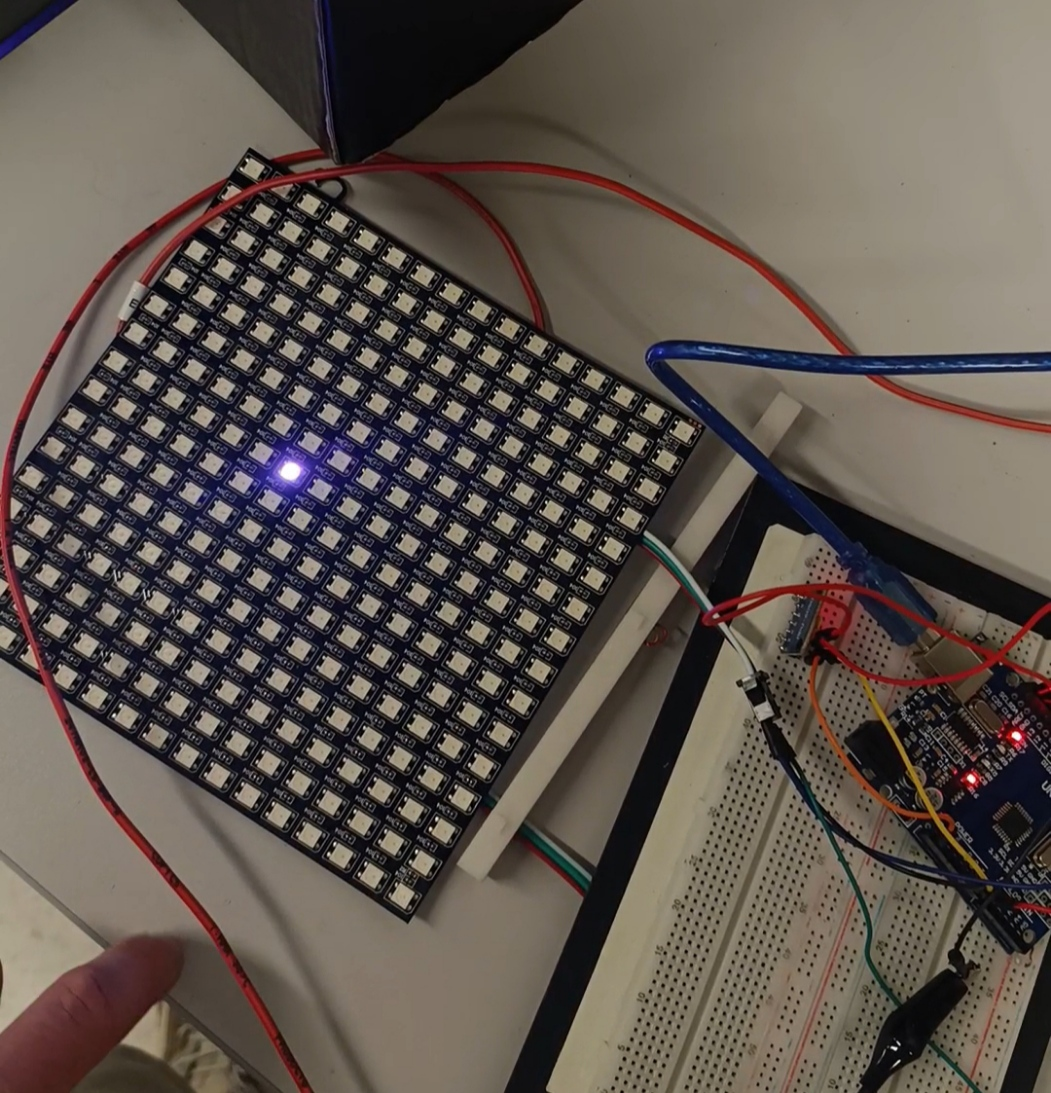
\includegraphics[width=0.45\textwidth]{anexos/4 Giroscopio/neutral.jpg}
    \caption{Funcionamiento general del sistema: LED en posición neutra con el sensor apoyado. Fuente: elaboración propia}
    \label{fig:WSneutral}
\end{figure}

El comportamiento al inclinar la protoboard mostró un desplazamiento suave sobre la matriz, acompañando correctamente la dirección del movimiento. Si bien se observó cierto \textit{jitter} en posiciones intermedias —debido al ruido natural del acelerómetro— este efecto fue menor comparado con la respuesta estable en movimientos más amplios, como inclinaciones pronunciadas o trayectorias circulares. La latencia del sistema fue baja y el retardo imperceptible, resultando en una interacción natural e intuitiva para el usuario.

\begin{figure}[H]
    \centering
    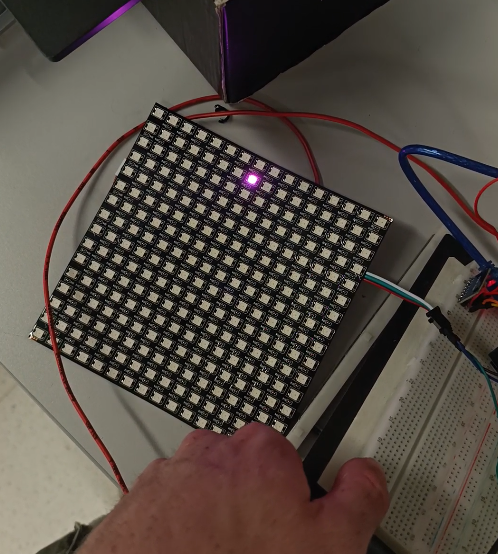
\includegraphics[width=0.45\textwidth]{anexos/4 Giroscopio/giroscopio2.png}
    \caption{Funcionamiento general del sistema: desplazamiento del LED al inclinar el MPU6050. Fuente: elaboración propia}
    \label{fig:WSinclinado}
\end{figure}

